\documentclass{article}
\usepackage[english]{babel}
\usepackage{csquotes}
\usepackage[
letterpaper,
top=2cm,
bottom=2cm,
left=3cm,
right=3cm,
marginparwidth=1.75cm
]{geometry}
\usepackage{amsmath}
\usepackage{graphicx}
\usepackage[
colorlinks=true, 
allcolors=blue]{hyperref}
\usepackage{multicol}
\usepackage{float}
\usepackage[affil-it]{authblk}

\usepackage[section]{placeins}
\usepackage{array}
\newcolumntype{P}[1]{>{\centering\arraybackslash}p{#1}}

\usepackage[
backend=biber,
style=nature
]{biblatex}

\addbibresource{paper_resources/bib.bib}

\title{\textbf{Applying U-Net for Medical Image Segmentation: A Case Study}}
\author{Carson Keller}
\affil{Department of Computer Science, Boise State University}
\date{}

\begin{document}
\maketitle

\begin{multicols}{2}

\section{Introduction}

In computer vision, image segmentation is the process of algorithmically partitioning an image into meaningful regions from which objects of interest are identified as defined by pixel characteristics relative to those regions \cite{palpal1993}. It serves many functions, including as a means to detect and isolate objects in autonomous driving systems or to compare and distinguish between likenesses in facial recognition applications. Notably, automated segmentation methods are an important development in medical image processing, providing the ability to automatically segregate and demarcate structures and other areas of interest across a range of radiological modalities, including ultrasound (US), computed tomography (CT), and magnetic resonance imaging (MRI).

Radiological imaging technology is a crucial tool for modern medicine in confirming diagnoses, informing prognoses, and aiding treatments. As its capability, accuracy, and resolution has increased, so too has its usefulness. The application of image segmentation to the robust field of radiology serves only to enhance those benefits. It poses the unique opportunity for augmenting and streamlining doctors’ workflows by providing computer-aided diagnoses, allowing better surgical planning and navigation, informing targeted treatments, and enabling enhanced efficiency, ultimately improving overall patient outcomes through revolutionized patient care \cite{realWorldApps}. When so many patients’ prognoses can be drastically impacted by these factors, when an early brain cancer diagnosis and quick, tailored treatment can mean the difference between death and survival, this technology has the potential to greatly impact the health and well-being of our society and communities, our friends and family, and, potentially, even ourselves.

This particular experiment serves as a case study, applying image segmentation methods to a dataset of MRI scan image files to assess the viability of this process as a proof of concept. Additionally, it also aims to evaluate the performance of different combinations and variations of deep learning models architectures, metrics, and loss functions informed by academic literature. This is done in the hope of finding a most successful, most performant composite model structure that yields the best results.

\section{Related work}
	
Traditional approaches to image segmentation include direct region detection methods \cite{rundo2016}, graph-based methods \cite{graphchen2018}, and active contour and level set models \cite{contourkhadidos2017}. Later approaches have attempted to adapt and apply traditional machine learning algorithms \cite{machinelearningrundo2020}, such as support vector machines (SVMs) \cite{svmswang2012} and unsupervised clustering \cite{clusteringren2019}. However, in recent years, more significant progress has been achieved utilizing deep learning models \cite{deepker2018} \cite{deeprueckert2020} \cite{deepcastiglioni2021}.

\begin{figure*}
\centering
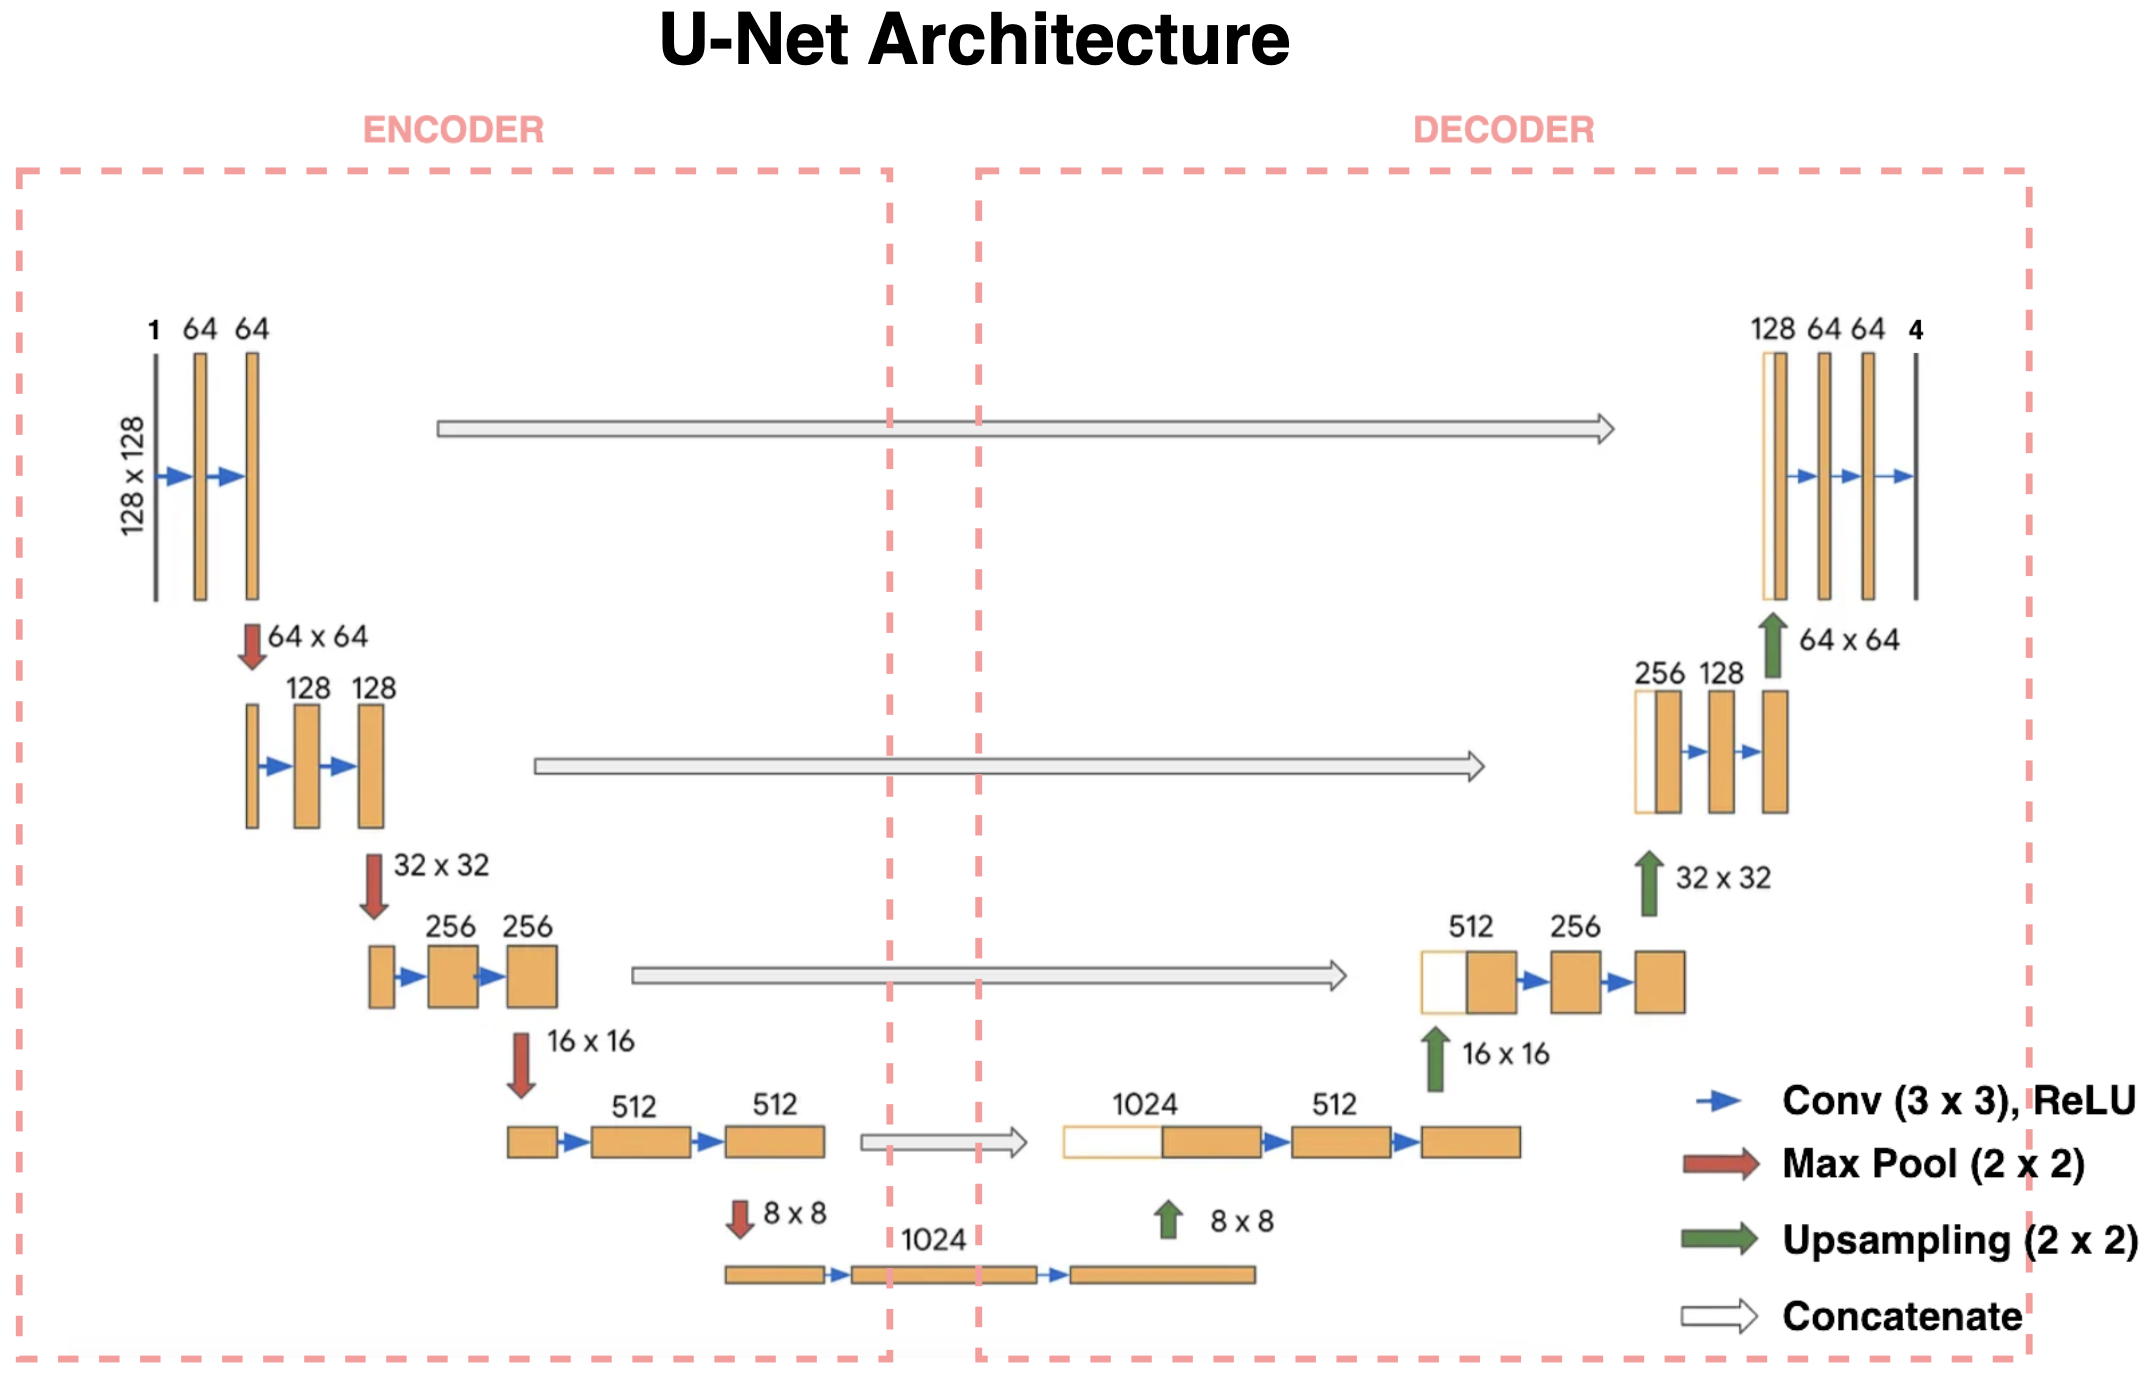
\includegraphics[width=0.85\linewidth]{paper_resources/u-net architecture.png}
\caption{\label{fig:u-net}Modified U-Net architecture with relevant input and output dimensions, layers, convolutional filter sizes, and other features accurate to this particular implementation.}
\end{figure*}

The most well-known deep learning model architecture for image segmentation, U-Net \cite{unet_ronneberger2015}, is the modification of the convolutional neural network (CNN) architecture into an encoder-decoder network. While CNNs alone have demonstrated significant performance when handling image input \cite{cnnClassification2012}, the hybridization of these two network types has yielded incredible efficacy in image segmentation applications. Through the use of convolutional layers, CNNs determine the presence of meaningful features and construct feature maps that are passed on to deeper layers in the model. Further, pooling layers allow dimensionality reduction, losing information but significantly reducing the overall number of parameters needed by the model. Implementing an encoder portion into the model architecture, as U-Net does, produces various feature maps or “hidden states” that capture the image input’s relevant characteristics and elements before combining them to generate a context vector, an “encoded” numeric matrix representation of the most important features. The decoder portion is then responsible for translating this context vector into a mask, or segmented version of the original image, maintaining the important features and segmenting the meaningful region as accurately as possible. This architecture thus enables end-to-end feature extraction and pixel classification. As depicted in Figure \ref{fig:u-net},  the structure of the baseline model is modified for this particular implementation, with accurate input and output dimensions, number of layers, convolutional filter sizes, and other features.

Different variations of the popular U-Net architecture have been developed, primarily specialized for different tasks. In image segmentation, specifically medical image segmentation, the most performant models beyond the base U-Net architecture have historically included variants of three principle categories: 3D U-Net, enabling 3-dimensional, volumetric segmentation \cite{3dUnet_2016}; Attention U-Net, allowing the ability to focus on areas of importance and ignore more unnecessary regions \cite{attentionUnet_2018}; and Residual U-Net, hybridizing the traditional U-Net model and the ResNet deep learning model and enabling it to overcome difficulty in training \cite{resUnet_2015}.

In training deep neural networks such as U-Net, backpropagation is used to update and optimize model parameters in accordance with the dictated loss function. Cross entropy loss, commonly used in classification applications, is used in the original U-Net implementation \cite{unet_ronneberger2015}. Other loss functions have been utilized, such as dice loss which is based on the common dice metric used for segmentation applications and is, therefore, a direct form of loss minimization. Generally, loss functions for image segmentation applications can be classified as distribution-based (such as cross entropy), region-based (such as dice loss), boundary-based (such as boundary loss), or as compound losses which combine multiple, independent loss functions \cite{comboLoss_taghanaki2019}. Generalizations of dice loss and cross entropy-based losses, such as unified focal loss for mitigating errors arising from class imbalance, have proven particularly robust and effecitve in medical image segmentation applications \cite{unifiedLoss_yeung2022}.
 
Choice of evaluation metric is just as critical as choice of loss function in deriving optimal performance from deep learning models. While loss functions adapt the model parameters during training, it is done with the purpose of ultimately optimizing chosen evaluation metrics. These metrics provide a holistic assessment of model performance after training is complete on validation and test data the model was not trained on. In image segmentation, common metrics include simple pixel accuracy (Rand index), precision and recall or the minimization of false positives and false negatives, respectively, the dice coefficient, the intersection-over-union value (IOU or Jaccard Index), and the Matthews correlation coefficient. Other proposed metrics include Otsu’s thresholding or the Coye and Grabcut algorithms, with the latter showing particular strength isolating skin lesions in medical image segmentation applications \cite{lesionMetrics_2020}. 

A predominant issue in medical image segmentation arises from class imbalance, or the significant, unequal distribution in area between meaningful foreground regions and their background. For example, foreground elements such as organs in automatic organ segmentation tend to be substantially smaller than the entire scan itself, resulting in a skewed distribution that favors background elements \cite{organSeg_roth2015}. This issue is significantly more prevalent in the realm of oncology where a tumor is usually even smaller than its organ of origin. This can be described as input imbalance whereas difficulty handling class imbalance resulting in classification errors arising during inference can be described as output imbalance \cite{comboLoss_taghanaki2019}. Such errors can include false positives and false negatives, respectively described as background pixels incorrectly included with the foreground region and foreground pixels incorrectly categorized with the background region and excluded from the foreground. Both errors are incredibly important in medical image segmentation as too many false positive pixels could significantly increase the target region’s area, leading to larger radiation fields or surgical margins, and too many false negatives could decrease the target region’s area, leading to inadequate radiation delivery or incomplete surgical excision.

\section{Methodology}

Through this experiment, image segmentation methods were applied to the BraTS2020 dataset of MRI scan image files to determine a baseline viability of this process as well as improve upon that baseline model, to the extent allowed by the availability of time and resources, to find the most successful, performant model possible and that yielded the best results.

\subsection{BraTS2020 Dataset}
	
This experiment utilized the BraTS2020 dataset, comprised of clinically-acquired pre-operative multimodal MRI scans of glioblastoma and lower grade glioma with pathologically confirmed diagnoses. All scan instances were available as NIfTI files (.nii.gz) in five treatment variations: 1. native (T1) and 2. post-contrast T1-weighted (T1Gd), 3. T2-weighted (T2), and 4. T2 Fluid Attenuated Inversion Recovery (T2-FLAIR) volumes, all of which were acquired from multiple institutions, with the fifth variation being a manually-derived segmentation. Each segmentation was a composite comprised of three partitions, annotations denoting the GD-enhancing tumor (ET — label 4), the peritumoral edema (ED — label 2), and the necrotic and non-enhancing tumor core (NCR/NET — label 1) \cite{bratsPaper}. From the 369 scans provided, 250 were utilized for training, 74 for validation, and 45 were reserved as test scans for model evaluation. Each scan file had a native image resolution of $240\times240$ pixels, with 155 voxels or slices to be examined. Due to variation in the first and last five slices in some of the scan files, processing was limited to voxels 5-150, or the middle 145 slices, of each scan file. Preparing each slice for input results in input dimensionality of $128\times128\times2$.

\subsection{Deep Learning Model}

Given its reputation for high performance in image segmentation, the traditional U-Net architecture was implemented as a baseline to assess performance of subsequent model variants. Upon establishing baseline metric values, the baseline model was modified, with various model features applied systematically to determine their respective impact on model performance with the ultimate goal of achieving the highest model metrics with the most accurate inferences. Such model variants were generated by alternating the activation function that determines each node’s output between ReLU and PReLU, the latter of which has shown promise in other medical image segmentation applications \cite{prelu_2020}, adding various numbers of dropout layers and passing a range of values to determine the proportion of nodes to drop, and including or excluding normalization layers between convolutional layers.

\begin{figure*}
\centering
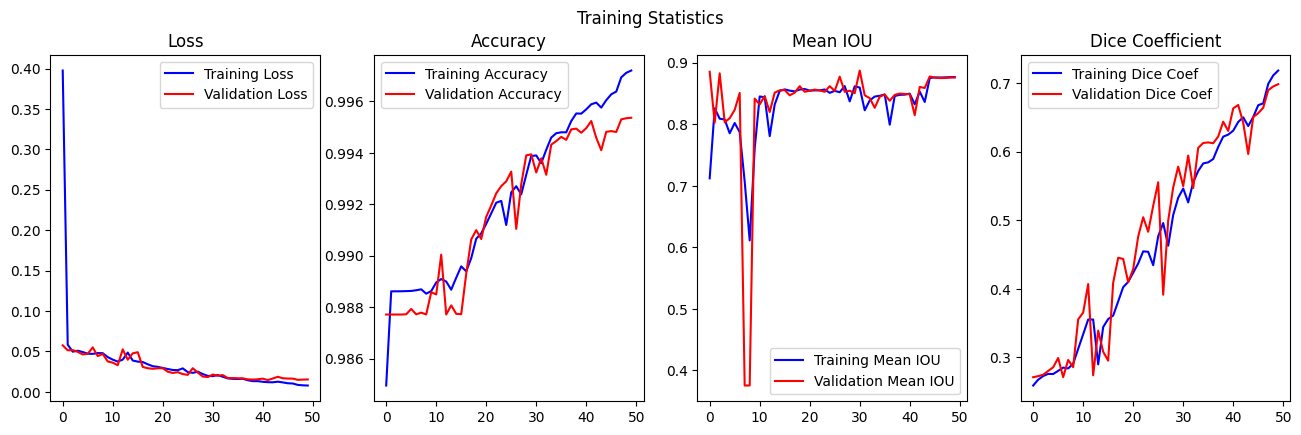
\includegraphics[width=1\linewidth]{paper_resources/training statistics.png}
\caption{\label{fig:train_stats}Most performant model loss, accuracy, mean IOU, and dice coefficient metrics from training and validation.}
\end{figure*}

\subsection{Loss Functions}
	
Motivated by the original U-Net implementation, the initial choice of loss function was the distribution-based categorical cross entropy loss \cite{unet_ronneberger2015}. This loss function is ideal for its ease of implementation and optimization but might have a potentially deleterious impact on performance with significantly imbalanced data. Thus, it constituted a sufficient baseline to measure other, potentially more effective, loss functions against. Had time allowed, other such loss functions to implement might have included unified focal loss which generalizes dice loss and cross entropy loss to mitigate issues that arise due to class imbalance, a loss function that has demonstrated to be quite effective in medical image segmentation applications \cite{unifiedLoss_yeung2022}. However, due to time constraints, computational demands of training, and hardware limitations, the ability to implement other loss functions beyond categorical cross entropy were out of reach.

\subsection{Evaluation Metrics}
	
Opting, instead, to examine the impact of model architecture variants and various loss functions in lieu of various evaluation metrics, hypothesizing they would have a greater impact on overall model performance, traditional metrics were chosen to evaluate the model throughout each trial. Accuracy, mean IOU, and dice coefficient (equations \ref{eq:acc}, \ref{eq:iou}, and \ref{eq:dice}, respectively) were all provided to the model for consideration as it optimized its parameters using its specified loss function. These metrics were held as constant throughout the entirety of experimentation despite adjusting other features and model parameters.

\begin{equation}
accuracy=\frac{TP+TN}{TP+TN+FP+FN}
\label{eq:acc}
\end{equation}
\begin{equation}
meanIOU=\frac{1}{n}\times\frac{TP}{TP+FP+FN}
\label{eq:iou}
\end{equation}
\begin{equation}
dice=\frac{2\times TP}{(2\times TP)+FP+FN}
\label{eq:dice}
\end{equation}

\subsection{Implementation}

Due to this experiment’s computational demands and limitations of local hardware availability, the processing of this experiment was conducted using GPU hardware acceleration available through Google’s online python coding environment, Colab. This allowed access to remote hardware resources and exponentially faster processing. Each training epoch on local, non-GPU-accelerated hardware took between 5 and 6 hours whereas offloading training and validation onto a remote GPU resource shortened that time to approximately 210 seconds per epoch, allowing the completion of a full, 50-epoch training session to be completed in just under 3 hours. The use of such resources is highly recommended if reprocessing is to be attempted as the computational demand of training this model and its variants is incredibly high.

\section{Experiment \& Results}

\begin{center}
\begin{table*}
\centering
\begin{tabular}{ |P{2cm}||P{1.5cm}|P{2cm}|P{2cm}|P{3cm}|  }
\multicolumn{5}{c}{\textbf{U-Net Implementation Statistics}} \\
\hline
\textbf{} & \textbf{Loss} & \textbf{Accuracy} & \textbf{Mean IOU} & \textbf{Dice Coefficient} \\
\hline
Training & 0.78\% & 99.72\% & 87.66\% & 71.80\% \\
\hline
Validation & 1.53\% & 99.54\% & 87.60\% & 69.81\% \\ 
\hline
Test & 1.78\% & 99.42\% & 82.00\% & 66.15\% \\
\hline
\end{tabular}
\caption{\label{tab:u-net stats table}Resulting evaluation metrics after training, validation, and testing of standard U-Net implementation.}
\end{table*}
\end{center}

\begin{figure*}[b]
\centering
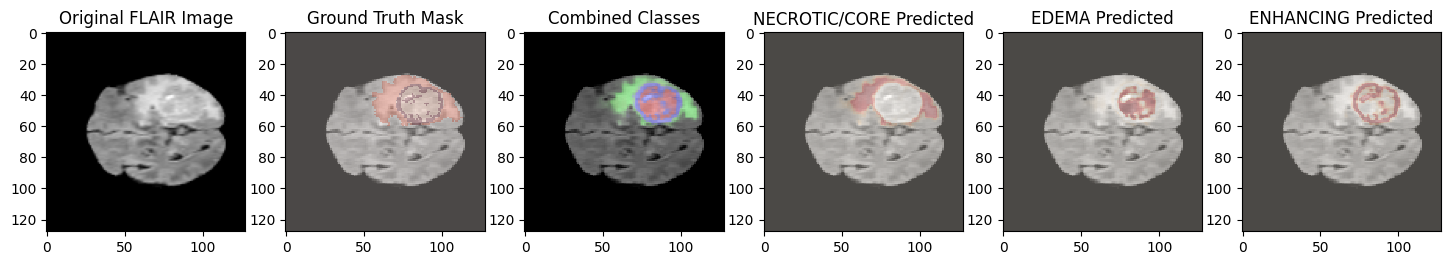
\includegraphics[width=1\linewidth]{paper_resources/example result.png}
\caption{\label{fig:ex_result}Original FLAIR image and manually segmented mask compared to class-by-class generated masks and combined composite mask.}
\end{figure*}

Comparing the results of the different model variants generated and tested, the outcomes were notably unremarkable. None of the predetermined modifications majorly improved or decreased performance of the model. That is, model performance was relatively consistent regardless of the activation function chosen, regardless of the inclusion or exclusion of dropout layers, the number of dropout layers included, or the coefficient for the dropout proportion selected, and regardless of the inclusion of normalization layers. All final pixel accuracy metric values came within 0.5\% of the simple, traditional U-Net architecture implementation, utilizing cross-entropy loss, that yielded the best results in terms of pixel accuracy with an impressive 99.42\% on the test data. These results reaffirm the performance of the U-Net architecture and suggest the need for further exploration regarding model-only optimization. That is to say, if one seeks to derive major improvement from a model alone, an entirely different model architecture may be more likely to provide more significant results than slightly augmenting or minorly modifying features in one’s current model architecture. Further, these results suggest substituting loss function or implementing some other more major changes to the experiment structure rather than lesser modifications to one’s current model architecture might yield a more significant impact on model performance.

For the sake of completing this case study though, upon finding no improvement after the attempted feature modifications beyond the standard U-Net implementation, that baseline model was assumed for the remainder of the procedure. The statistics generated in its training, validation, and testing were logged and graphed. Examining these statistics from its training run, epoch-to-epoch, as depicted in Figure \ref{fig:train_stats},  U-Net displayed its strengths, with performance in each metric steadily moving in the desired direction. Aside from some more drastic variance in the Mean IOU values, loss, accuracy, and dice coefficient values trend fairly consistently. The final, resultant numeric values of each metric are noted in Table \ref{tab:u-net stats table}.

Out of context, such high pixel accuracy scores fail to convey the significance of the seemingly negligible 0.58\% error remaining. However, when an inference is made and a mask is generated and compared to the manually segmented ground truth mask, differences become clear with even that degree of error. Such can be seen in Figure \ref{fig:ex_result}. 

While the derived mask is primarily true to form, false positive and false negative pixels, pixels incorrectly included with the foreground or background, respectively, become noticeable. In certain areas, the mask stretches beyond its border, but in others, it atrophies.  It is true that the general shape is true to form and primarily accurate. However, that 0.58\% error remaining comes into stark relief at the margins and boundaries.

Despite the general success and capability of this technology, this insufficiency only yields further reason to continue this work. There is only room but to improve. With technology as capable as this and with countless avenues yet unexplored, including many potential optimization tactics named within this work itself, there is a path forward and progress to make, for science, for medicine, for doctors, and for patients the world over.

\FloatBarrier

\end{multicols}

\printbibliography

\end{document}
